\section{Model description}

\subsection{F-16 model}

  This section aims to present the reduced equations for the dynamics of the F-16 fixed-wing aircraft which simulated in a non-linear manner using SIDPAC software.

  \subsubsection{Mathematical models of aircrafts}

  The notation for the aircraft is the one shown in Figure \ref{fig:aircraftNotation}.

  \begin{figure}[!htpb]
    \centering
    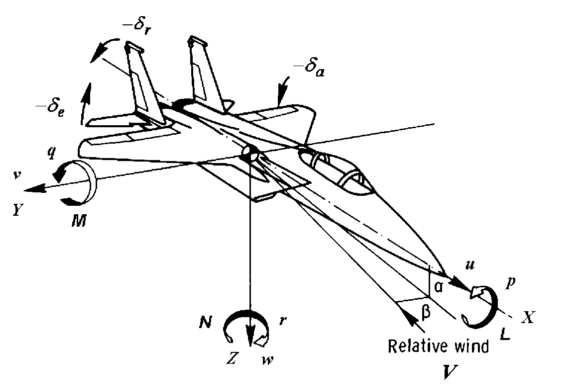
\includegraphics[width=0.7 \textwidth]{figures/aircraftNotation}
    \caption[Airplane notation and sign conventions]{Airplane notation and sign conventions: u, v, w 5 body-axis components of aircraft velocity relative to Earth axes; $p$, $q$, $r$ 5 body-axis components of aircraft angular velocity; $X$, $Y$, $Z$ 5 body-axis components of aerodynamic force acting on the aircraft; and $L$, $M$, $N$ 5 body-axis components of aerodynamic moment acting on the aircraft.}
    \label{fig:aircraftNotation}
  \end{figure}

  The components of the aerodynamic forces and moments, are the following:

  \noindent
  Forces:
  \begin{eqnarray}
  \mathrm{Body \quad axes} \qquad && \mathrm{Stability \quad axes} \\ [6pt]
  X = \bar{q}SC_X \qquad && D = \bar{q}SC_D \\ [6pt]
  Z = \bar{q}SC_Z \qquad && L = \bar{q}SC_L \\ [6pt]
  Y = \bar{q}SC_Y \qquad && Y = \bar{q}SC_Y
  \end{eqnarray} 

  \noindent
  Moments:
  \begin{eqnarray}
  L = \bar{q} b S C_l \\ [6pt]
  M = \bar{q} \bar{c} S C_m \\ [6pt]
  N = \bar{q} b S C_n
  \end{eqnarray}

  \noindent
  where $\bar{q}=1/2 \rho V^2$ is the dynamic pressure, $\rho$ is the air density, $V$ is the airspeed, $S$ is the wing reference area, $b$ is the wing span and $\bar{c}$ is the mean aerodynamic chord (MAC). 

  The forces expressed in the wind axis systems as shown in set Equations \ref{eq:aeroForcesInWingAxis}. 

  \begin{eqnarray} \label{eq:aeroForcesInWingAxis}
  \msub{C}{L} = - \msub{C}{Z} \cos \alpha + \msub{C}{X} \sin \alpha \nonumber \\[6pt]
  \msub{C}{D} = - \msub{C}{X} \cos \alpha - \msub{C}{Z} \sin \alpha
  \end{eqnarray}

  The Taylor expansion for the longitudinal motion of the aircraft are expressed in set of Equations \ref{eq:LongitudinalFixedWing}.

  \begin{eqnarray} \label{eq:LongitudinalFixedWing}
  C_D &=& C_{D_0} + C_{D_V} \frac{\Delta V}{V_0} + C_{D_\alpha} \Delta \alpha + C_{D_q} \frac{q \bar{c}}{2 V_0} + C_{D_{\msub{\delta}{e}} }\Delta \msub{\delta}{e} \nonumber \\ [6pt]
  C_L &=& C_{L_0} + C_{L_V} \frac{\Delta V}{V_0} + C_{L_\alpha} \Delta \alpha + C_{L_{\dot{\alpha}}} \frac{\dot{\alpha} \bar{c} }{2 V_0} + C_{L_q} \frac{q \bar{c}}{2 V_0} + C_{L_{\msub{\delta}{e}}} \msub{\delta}{e} \nonumber \\ [6pt]
  C_m &=& C_{m_0} + C_{m_V} \frac{\Delta V}{V_0} + C_{m_\alpha} \Delta \alpha + C_{m_{\dot{\alpha}}} \frac{\dot{\alpha} \bar{c} }{2 V_0} + C_{m_q} \frac{q \bar{c}}{2 V_0} + C_{m_{\msub{\delta}{e}}} \msub{\delta}{e} 
  \end{eqnarray}

  The set of equations that describe the motion of the aircraft, obtained from the Taylor series expansion is the one represented in Equation \ref{eq:LateralFixedWing}.

  \begin{eqnarray} \label{eq:LateralFixedWing}
  C_Y &=& C_{Y_0} + C_{Y_\beta}\Delta\beta + C_{Y_p}\frac{pb}{2V_0} + C_{Y_r}\frac{rb}{2V_0} + C_{Y_{\msub{\delta}{a}} }\Delta \msub{\delta}{a} + C_{Y_{\msub{\delta}{r}} }\Delta \msub{\delta}{r} \nonumber \\ [6pt]
  C_l &=& C_{l_0} + C_{l_\beta}\Delta\beta + C_{l_p}\frac{pb}{2V_0} + C_{l_r}\frac{rb}{2V_0} + C_{l_{\msub{\delta}{a}} }\Delta \msub{\delta}{a} \qquad (C_{l_{\msub{\delta}{r}}} \ll 1) \nonumber \\ [6pt]
  C_n &=& C_{n_0} + C_{n_\beta}\Delta\beta + C_{n_p}\frac{pb}{2V_0} + C_{n_r}\frac{rb}{2V_0} + C_{n_{\msub{\delta}{r}} }\Delta \msub{\delta}{r} \qquad (C_{l_{\msub{\delta}{a}}} \ll 1)
  \end{eqnarray}

\subsection{Helicopter model}

  \subsubsection{Model forces and moments coefficients}
    Forces: 
    $$
    X_u, X_v, X_w, X_p, X_q, X_r \\
    Y_u, Y_v, Y_w, Y_p, Y_q, Y_r \\
    Z_u, Z_v, Z_w, Z_p, Z_q, Z_r
    $$

    Moments:
    $$
    L_u, L_v, L_w, L_p, L_q, L_r \\
    M_u, M_v, M_w, M_p, M_q, M_r \\
    N_u, N_v, N_w, N_p, N_q, N_r
    $$

    Controllability, $\mat{G}$ matrix:
    Forces
    $$
    X_{\theta_{\mathrm{lon}}}, X_{\theta_{\mathrm{lat}}}, X_{\theta_{\mathrm{ped}}}, X_{\theta_{\mathrm{col}}} \\
    Y_{\theta_{\mathrm{lon}}}, Y_{\theta_{\mathrm{lat}}}, Y_{\theta_{\mathrm{ped}}}, Y_{\theta_{\mathrm{col}}} \\
    Z_{\theta_{\mathrm{lon}}}, Z_{\theta_{\mathrm{lat}}}, Z_{\theta_{\mathrm{ped}}}, Z_{\theta_{\mathrm{col}}}
    $$

    Moments
    $$
    M_{\theta_{\mathrm{lon}}}, M_{\theta_{\mathrm{lat}}}, M_{\theta_{\mathrm{ped}}}, M_{\theta_{\mathrm{col}}} \\
    N_{\theta_{\mathrm{lon}}}, N_{\theta_{\mathrm{lat}}}, N_{\theta_{\mathrm{ped}}}, N_{\theta_{\mathrm{col}}} \\
    N_{\theta_{\mathrm{lon}}}, N_{\theta_{\mathrm{lat}}}, N_{\theta_{\mathrm{ped}}}, N_{\theta_{\mathrm{col}}}
    $$

    Time delays
    $$
    \tau_{\mathrm{lon}}, \tau_{\mathrm{lat}}, \tau_{\mathrm{ped}}, \tau_{\mathrm{col}}
    $$

  \subsubsection{Equations of motion for a linearised model}

    The linearisation of forces and moments by means of the small perturbation theory about the body axes centre leads to:

    \begin{eqnarray}
      X &=& m \{\dot{u} + q W_e -d_x(q^2 + r^2) + d_y(pq - \dot{r}) + d_z(pr + \dot{q}) \} \\[6pt]
      Y &=& m \{ \dot{v} - p W_e + r U_e + d_x(pq + \dot{r}) - d_y(p^2 + r^2) + d_z(qr - \dot{p}) \} \\[6pt]
      Z &=& m \{\dot{w} - q U_e + d_x(pr - \dot{q}) + d_y(qr + \dot{p}) + d_z(p^2 + q^2) \} \\[6pt]
      L &=& I_{xx} \dot{p} - I_{xz}\dot{r} - Y d_z + Z d_y \\[6pt]
      M &=& I_{yy} \dot{q} - Z d_x + X d_z \\[6pt]
      N &=& I_{zz} \dot{r} - I_{xz} \dot{p} - X d_y +Y d_x
    \end{eqnarray}

    And, considering the forces and moments arise from aerodynamic, gravitational and control sources, it can be written that:

    \begin{eqnarray}
      X &=& u \mathring{X}_u + w \mathring{X}_w + q \mathring{X}_q - \theta m g \cos \theta_e + \theta_{\mathrm{lon}} \mathring{X}_{\theta_{\mathrm{lon}}} + \theta_{\mathrm{col}} \mathring{X}_{\theta_{\mathrm{col}}} \\[6pt]
      Y &=& v \mathring{Y}_v + p \mathring{Y}_p + r \mathring{Y}_r + \phi m g \sin \theta_e + \psi m g \cos \theta_e + \theta_{\mathrm{lat}} \mathring{Y}_{\theta_{\mathrm{lat}}} + \theta_{\mathrm{ped}} \mathring{Y}_{\theta_{\mathrm{ped}}} \\[6pt]
      Z &=& u \mathring{Z}_u + w \mathring{Z}_w + q \mathring{Z}_q - \theta m g \sin \theta_e + \theta_{\mathrm{lon}} \mathring{Z}_{\theta_{\mathrm{lon}}} + \theta_{\mathrm{col}} \mathring{Z}_{\theta_{\mathrm{col}}} \\[6pt]
      L &=& v \mathring{L}_v + p \mathring{L}_p + r \mathring{L}_r + \theta_{\mathrm{lat}} \mathring{L}_{\theta_{\mathrm{lat}}} + \theta_{\mathrm{ped}} \mathring{L}_{\theta_{\mathrm{ped}}} + \theta_{\mathrm{lon}} \mathring{L}_{\theta_{\mathrm{lon}}}\\[6pt] %lon added here
      M &=& u \mathring{M}_u + w \mathring{M}_w + q \mathring{M}_q + \theta_{\mathrm{lon}} \mathring{M}_{\theta_{\mathrm{lon}}} + \theta_{\mathrm{col}} \mathring{M}_{\theta_{\mathrm{col}}} + \theta_{\mathrm{ped}} \mathring{M}_{\theta_{\mathrm{ped}}} + \theta_{\mathrm{lat}} \mathring{M}_{\theta_{\mathrm{lat}}}\\[6pt] %pedal and lat added here
      N &=& v \mathring{N}_v + p \mathring{N}_p + r \mathring{N}_r + \theta_{\mathrm{lat}} \mathring{N}_{\theta_{\mathrm{lat}}} + \theta_{\mathrm{ped}} \mathring{N}_{\theta_{\mathrm{ped}}}
    \end{eqnarray}

  \subsubsection{Longitudinal and lateral dynamics from the linearized model}

    The linearized model for longitudinal dynamics results on:

    \begin{eqnarray}
      \left[ \begin{array}{c} \dot{u} \\ \dot{w} \\ \dot{q} \\ \dot{\theta} \end{array} \right] &=& \mat{A} \left[ \begin{array}{c} u \\ w \\ q \\ \theta \end{array} \right] + \mat{B} \left[ \begin{array}{c} \theta_{\mathrm{col}} \\ \theta_{\mathrm{lon}} \end{array} \right] \\[6pt]
      \mat{y} &=& \mat{C} \left[ \begin{array}{c} u \\ w \\ q \\ \theta \end{array} \right] + \mat{D} \left[ \begin{array}{c} \theta_{\mathrm{col}} \\ \theta_{\mathrm{lon}} \end{array} \right]
    \end{eqnarray}

    Ultimately, this will result in the following characteristic equation: $$(T_1 s + 1) ( T_2 s + 1) / (s^2 + 2\zeta \omega_n s + \omega_n^2) = 0$$

    And for the lateral, results on:

    \begin{eqnarray}
      \left[ \begin{array}{c} \dot{v} \\ \dot{p} \\ \dot{r} \\ \dot{\phi} \end{array} \right] &=& \mat{A} \left[ \begin{array}{c} v \\ p \\ r \\ \phi \end{array} \right] + \mat{B} \left[ \begin{array}{c} \theta_{\mathrm{lat}} \\ \theta_{\mathrm{ped}} \end{array} \right] \\[6pt]
      \mat{y} &=& \mat{C} \left[ \begin{array}{c} v \\ p \\ r \\ \phi \end{array} \right] + \mat{D} \left[ \begin{array}{c} \theta_{\mathrm{lat}} \\ \theta_{\mathrm{ped}} \end{array} \right]
    \end{eqnarray}

    Ultimately, this will result in the following characteristic equation for the lateral/directional motion: $$(T_1 s + 1) ( T_2 s + 1) / (s^2 + 2\zeta \omega_n s + \omega_n^2) s = 0$$